\documentclass[greek]{beamer}
%\usepackage{fontspec}
\usepackage{amsmath,amsthm}
\usepackage{unicode-math}
\usepackage{xltxtra}
\usepackage{graphicx}
\usetheme{CambridgeUS}
\usecolortheme{seagull}
\usepackage{hyperref}
\usepackage{ulem}
\usepackage{xgreek}

\usepackage{pgfpages}
\usepackage{tikz}
\usepackage{tkz-tab}
%\setbeameroption{show notes on second screen}
%\setbeameroption{show only notes}

\setsansfont{Noto Serif}

\usepackage{multicol}

\usepackage{appendixnumberbeamer}

\usepackage{polynom}

\usepackage{pgffor}

\setbeamercovered{transparent}
\beamertemplatenavigationsymbolsempty

\title{Κωνικές Τομές}
\subtitle{Παραβολή}
\author[Λόλας]{Κωνσταντίνος Λόλας}
\date{}

\begin{document}

\begin{frame}
  \titlepage
\end{frame}

\section{Θεωρία}
\begin{frame}{Γεωμετρικοί τόποι παντού}
  Κάναμε
  \begin{enumerate}
    \item<1-> σταθερή απόσταση από ένα σημείο
    \item<2-> ίση απόσταση από δύο σημεία
    \item<3-> σταθερή απόσταση από ευθεία
    \item<4-> ίση απόσταση από δύο ευθείες
  \end{enumerate}
  \only<5> {άρα το επόμενο, μοιραία θα είναι το} \only<6> {\emph{ίση απόσταση από σημείο και ευθεία?}}
\end{frame}

\begin{frame}{Φύγαμε για Geogebra}
  \href{https://www.geogebra.org/classic/wfmc8s24}{\beamergotobutton{Geogebra}}
\end{frame}

\begin{frame}{Λίγο πιο απλά?}
  Φυσικά. Θα ασχοληθούμε μόνο με τις παραβολές που έχουν:
  \begin{itemize}
    \item εστία πάνω στους άξονες
    \item διευθετούσα κάθετη στον άξονα της εστίας
    \item η αρχή των αξόνων είναι στο μέσο της εστίας και της διευθετούσας
  \end{itemize}
\end{frame}

\begin{frame}{Ακόμα πιο απλά?}
  Και πάλι φυσικά.
  \begin{itemize}
    \item Εστία $Ε(\dfrac{p}{2},0)$
    \item Διευθετούσα $x=-\dfrac{p}{2}$
  \end{itemize}
  ή
  \begin{itemize}
    \item Εστία $Ε(0,\dfrac{p}{2})$
    \item Διευθετούσα $y=-\dfrac{p}{2}$
  \end{itemize}
\end{frame}

\begin{frame}[label=Παραβολή]{Πιο επίσημα?}
  \begin{block}{Εξίσωση Παραβολής 1}
    Η παραβολή με εστία το σημείο $Ε(\dfrac{p}{2},0)$ και διευθετούσα $x=-\dfrac{p}{2}$ έχει εξίσωση
    $$y^2=2px$$
  \end{block}

  \hyperlink{ΑπόδειξηΕξίσωσης}{\beamerbutton{Πάμε για απόδειξη?}}

\end{frame}

\begin{frame}{Πρώτες παρατηρήσεις}
  \begin{itemize}
    \item<1-> Το σημείο $(0,0)$ ανήκει πάντα στην παραβολή
    \item<2-> ο $y'y$ είναι άξονας συμμετρίας
    \item<3-> η συνάρτηση $f(x)=\sqrt{x}$ είναι ο "πάνω" κλάδος της παραβολής
  \end{itemize}
\end{frame}

\begin{frame}{Τα ίδια, αλλά ανάποδα!}
  Αλλάξτε τα $x$ με τα $y$!
  \begin{block}{Εξίσωση Παραβολής 2}
    Η παραβολή με εστία το σημείο $Ε(0,\dfrac{p}{2})$ και διευθετούσα $y=-\dfrac{p}{2}$ έχει εξίσωση
    $$x^2=2py$$
  \end{block}
\end{frame}

\begin{frame}{Πρώτες παρατηρήσεις 2}
  \begin{itemize}
    \item<1-> Το σημείο $(0,0)$ ανήκει πάντα στην παραβολή
    \item<2-> ο $x'x$ είναι άξονας συμμετρίας
    \item<3-> η συνάρτηση $f(x)=x^2$ είναι μια παραβολή
  \end{itemize}
\end{frame}

\begin{frame}[label=Εφαπτόμενη]{Εφαπτομένη παραβολής}
  \begin{block}{Εξίσωση}
    Η εξίσωση της εφαπτομένης της παραβολής $y^2=2px$ στο σημείο της $(x_1,y_1)$ είναι η $$yy_1=p(x+x_1)$$
  \end{block}

  \hyperlink{ΑπόδειξηΕφαπτόμενη}{\beamerbutton{Πάμε για απόδειξη?}}
\end{frame}

\begin{frame}[label=Ιδιότητες]{Ιδιότητες Παραβολής $y^2=2px$}
  \begin{enumerate}
    \item<1-> Η εφαπτομένη της στο σημείο της $(x_1,y_1)$ τέμνει τον άξονα στο σημείο $(-x_1,0)$
    \item<2-> Κάθε παράλληλη στον $x'x$ ανακλάται στην παραβολή και περνά από την εστία
  \end{enumerate}

  \only<1>{\hyperlink{Απόδειξη1}{\beamerbutton{Πάμε για απόδειξη?}}}
  \only<2>{\hyperlink{Απόδειξη2}{\beamerbutton{Πάμε για απόδειξη?}}}
\end{frame}

\section{Ασκήσεις}
\begin{askisi}
  Να βρείτε την εξίσωση της παραβολής που έχει κορυφή την αρχή των αξόνων και επιπλέον:
  \begin{enumerate}
    \item<1-> έχει άξονα συμμετρίας τον άξονα $x'x$ και εστία $Ε(3,0)$
    \item<2-> έχει άξονα συμμετρίας τον άξονα $x'x$ και διευθετούσα $δ:x=4$
    \item<3-> έχει άξονα συμμετρίας τον άξονα $y'y$ και εστία $Ε(0,-2)$
    \item<4-> έχει άξονα συμμετρίας τον άξονα $y'y$ και η απόσταση της εστίας $Ε$ από την διευθετούσα $δ$ είναι $2$
  \end{enumerate}

  % \hyperlink{Λύση1}{\beamerbutton{Λύση}}

\end{askisi}

\begin{askisi}
  Να βρείτε την εστία $Ε$ και τη διευθετούσα $δ$ της παραβολής με εξίσωση:
  \begin{enumerate}
    \item<1-> $y^2=3x$
    \item<2-> $y=-2x^2$
  \end{enumerate}

  % \hyperlink{Λύση2}{\beamerbutton{Λύση}}

\end{askisi}

\begin{askisi}
  Να βρείτε την εξίσωση της εφαπτομένης της παραβολής $C:y^2=4x$, που είναι κάθετη στην ευθεία $ε:x+2y+1=0$
  \begin{enumerate}
    \item<1-> $Α(3,4)$
    \item<2-> $Β(-4,μ)$, $μ>0$
  \end{enumerate}

  % \hyperlink{Λύση3}{\beamerbutton{Λύση}}

\end{askisi}

\begin{askisi}
  Δίνεται η παραβολή $C:y^2=2x$. Να βρείτε την εφαπτομένη της παραβολής που διέρχεται από το σημείο $Α(-4,1)$

  % \hyperlink{Λύση4}{\beamerbutton{Λύση}}

\end{askisi}

\begin{askisi}
  Να βρείτε την εξίσωση της παραβολής $C$, που έχει κορυφή την αρχή των αξόνων, άξονα συμμετρίας τον $x'x$ και εφάπτεται της ευθείας $ε:2x-y+4=0$

  % \hyperlink{Λύση5}{\beamerbutton{Λύση}}

\end{askisi}

\begin{askisi}
  Δίνεται η παραβολή $C_1:y^2=4x$ και ο κύκλος $C_2:x^2+y^2=\frac{1}{2}$.
  \begin{enumerate}
    \item<1-> Να δείξετε ότι η εφαπτόμενη $ε$ της παραβολής $C_1$ στο σημείο της $Α(1,μ)$, $μ>0$ εφάπτεται στον κύκλο $C_2$
    \item<2-> Αν η ευθεία $ε$ του προηγούμενου ερωτήματος τέμνει τον άξονα $x'x$ στο $Β$, να βρείτε την άλλη κοινή εφαπτόμενη $η$ του κύκλου $C_2$ και της παραβολής $C_1$, καθώς και το σημείο επαφής της $C_1$ με την $η$
  \end{enumerate}

  % \hyperlink{Λύση6}{\beamerbutton{Λύση}}

\end{askisi}

\begin{askisi}
  Δίνεται η παραβολή $C:y^2=4x$. Να βρείτε την εξίσωση της χορδής της $C$ που έχει μέσο το σημείο $Μ(2,-1)$

  %\hyperlink{Λύση7}{\beamerbutton{Λύση}}

\end{askisi}

\begin{askisi}
  Δίνεται η παραβολή $y^2=2x$. Να δείξετε ότι τα μέσα $Μ$ των χορδών που είναι παράλληλες στην ευθεία $ε:x-y+1=0$, βρίσκονται σε ημιευθεία.

  %\hyperlink{Λύση8}{\beamerbutton{Λύση}}

\end{askisi}

\begin{askisi}
  Δίνεται η ευθεία $ε:x-2y+6=0$, ο κύκλος $C_1:x^2+y^2+4x+3=0$ και η παραβολή $C_2:y^2=x$. Έστω ένα σημείο $Μ$ που κινείται στην παραβολή.
  \begin{enumerate}
    \item<1-> Να δείξετε ότι $(ΜΝ)\ge \sqrt{5}$, όπου $Ν$ σημείο της ευθείας
    \item<2-> Να βρείτε το πλησιέστερο σημείο της παραβολής $C_2$ από την ευθεία $ε$
    \item<3-> Να δείξετε ότι $(ΜΡ)\ge 1$, όπου $Ρ$ σημείο του κύκλου
  \end{enumerate}

  %\hyperlink{Λύση9}{\beamerbutton{Λύση}}

\end{askisi}

\appendix

\section{}
\begin{frame}
  Στο moodle θα βρείτε τις ασκήσεις που πρέπει να κάνετε, όπως και αυτή τη παρουσίαση
\end{frame}

\section{Αποδείξεις}
\begin{frame}[label=ΑπόδειξηΕξίσωσης]{Απόδειξη εξίσωσης Παραβολής}
  Η εστία είναι η $Ε(\frac{p}{2},0)$ και η διευθετούσα $ε:x=-\frac{p}{2}$. Για κάθε σημείο $M(x,y)$ θα ισχύει:
  $$|ME|=d_{(ε,M)}$$
  \begin{gather*}
    \sqrt{\left(x-\frac{p}{2}\right)^2+(y-0)^2}=\dfrac{|1\cdot x+0\cdot y+\frac{p}{2}|}{\sqrt{1^2+0^2}} \\ \pause
    \sqrt{\left(x-\frac{p}{2}\right)^2+y^2}=|x+\frac{p}{2}| \\ \pause
    \left(   \sqrt{\left(x-\frac{p}{2}\right)^2+y^2}\right)^2=\left(   |x+\frac{p}{2}|\right)^2 \\ \pause
    x^2-px+\frac{p^2}{4}+y^2=x^2+px+\frac{p^2}{4} \\ \pause
    y^2=2px
  \end{gather*}

  \hyperlink{Παραβολή}{\beamerbutton{Πίσω στη θεωρία}}
\end{frame}

\begin{frame}[label=ΑπόδειξηΕφαπτόμενη]{Απόδειξη εφαπτόμενης}
  Η παραβολή έχει εξίσωση $y^2=2px$ και έστω σημείο της $M(x_1,y_1)$. Επιλέγουμε τυχαίο σημείο $A(x_2,y_2)$. Η εφαπτόμενη στο $Μ$ έστω είναι της μορφής $$y=λx+β$$
  \begin{gather*}
    λ=\dfrac{y_2-y_1}{x_2-x_1}  \text{ και αφού διέρχεται από το Μ}\\ \pause
    y-y_1=\dfrac{y_2-y_1}{x_2-x_1}(x-x_1)
  \end{gather*} \pause
  Για τα Μ και Α ισχύει:
  \begin{gather*}
    y_1^2=2px_1 \text{ και } y_2^2=2px_2 \\ \pause
    y_2^2-y_1^2=2p(x_2-x_1) \implies (y_2-y_1)(y_2+y_1)=2p(x_2-x_1)\implies \\ \pause
    \dfrac{y_2-y_1}{x_2-x_1}=\dfrac{2p}{y_2+y_1}
  \end{gather*}
\end{frame}

\begin{frame}{Απόδειξη εφαπτόμενης}
  Είχαμε $y-y_1=\dfrac{y_2-y_1}{x_2-x_1}(x-x_1)$
  και βρήκαμε $\dfrac{y_2-y_1}{x_2-x_1}=\dfrac{2p}{y_2+y_1}$.
  Άρα
  $$y-y_1=\dfrac{2p}{y_2+y_1}(x-x_1)$$
  Αν τώρα το $y_2$ τείνει στο $y_1$ θα έχουμε
  \begin{gather*}
    y-y_1=\dfrac{p}{y_1}(x-x_1) \\ \pause
    yy_1-y_1^2=px-px_1 \\ \pause
    yy_1-2px_1=px-px_1 \\ \pause
    yy_1=px+px_1 \\ \pause
    yy_1=p(x+x_1)
  \end{gather*}

  \hyperlink{Εφαπτόμενη}{\beamerbutton{Πίσω στη θεωρία}}
\end{frame}

\begin{frame}[label=Απόδειξη1]{Απόδειξη τομής εφαπτόμενης - άξονα}
  Στην
  $$yy_1=p(x+x_1)$$
  και για $y=0$, έχουμε
  $$0=p(x+x_1)\implies x=-x_1$$
  Άρα το σημείο $$Κ(-x_1,0)$$
  \hyperlink{Ιδιότητες}{\beamerbutton{Πίσω στη θεωρία}}
\end{frame}

\begin{frame}[label=Απόδειξη2]{Απόδειξη ανακλαστικής ιδιότητας}
  Θα δείξουμε ότι $|ΜΕ|=|ΝΕ|$
  \begin{gather*}
    \sqrt{\left( x_1-\frac{p}{2} \right)^2+(y_1-0)^2 }=\sqrt{x_1^2-px_1+\frac{p^2}{4}+y_1^2 } \\ \pause
    \sqrt{x_1^2-px_1+\frac{p^2}{4}+2px_1 }=\sqrt{x_1^2+px_1+\frac{p^2}{4} } \\ \pause
    \sqrt{\left( x_1+\frac{p}{2} \right)^2}=\left| \frac{p}{2}+x_1 \right|
  \end{gather*}

  \centering
  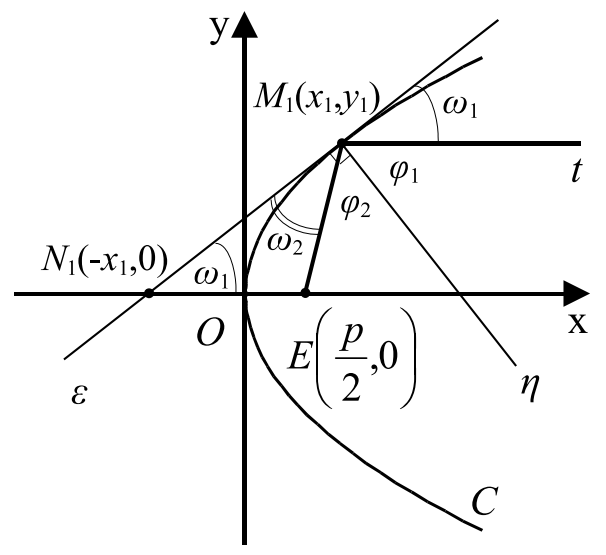
\includegraphics[width=0.3\textwidth]{"../images/reflection.png"}

  \hyperlink{Ιδιότητες}{\beamerbutton{Πίσω στη θεωρία}}
\end{frame}


% \section{Λύσεις Ασκήσεων}
% \begin{frame}
%  \tableofcontents
% \end{frame}
%
% \subsection{Άσκηση 1}
% \begin{frame}[label=Λύση1]
%  Με θεώρημα ενδιαμέσων τιμών. Η συνάρτηση είναι συνεχής στο $[10,11]$ με $f(10)=1024$ και $f(11)=2048$. Αφού $2023\in (1024,2048)$ υπάρχει $x_0$...
%
%  \hyperlink{Άσκηση1}{\beamerbutton{Πίσω στην άσκηση}}
% \end{frame}
%
% \subsection{Άσκηση 2}
% \begin{frame}[label=Λύση2]
%  Με Bolzano ή με μέγιστης ελάχιστης τιμής και ΘΕΤ.
%
%  \begin{gather*}
%   f(3)<f(2)<f(1) \\
%   3f(3)<f(1)+f(2)+f(3)<3f(1) \\
%   f(3)<\dfrac{f(1)+f(2)+f(3)}{3}<f(1)
%  \end{gather*}
%
%  \hyperlink{Άσκηση2}{\beamerbutton{Πίσω στην άσκηση}}
% \end{frame}
%
% \subsection{Άσκηση 3}
% \begin{frame}[label=Λύση3]
%  Προφανές ελάχιστο στα $x_1=1$ και $x_2=3$. Ως συνεχής στο $[1,3]$ έχει σίγουρα ΚΑΙ μέγιστο στο $(1,3)$
%
%  \hyperlink{Άσκηση3}{\beamerbutton{Πίσω στην άσκηση}}
% \end{frame}
%
% \subsection{Άσκηση 4}
% \begin{frame}[label=Λύση4]
%  Η συνάρτηση `απόστασης` $f(x)-x$ είναι ορισμένη στο κλειστό διάστημα και έχει σίγουρα μέγιστο
%
%  \hyperlink{Άσκηση4}{\beamerbutton{Πίσω στην άσκηση}}
% \end{frame}
%
% \subsection{Άσκηση 5}
% \begin{frame}[label=Λύση5]
%  Όμοια με την Άσκηση 2
%
%  \hyperlink{Άσκηση5}{\beamerbutton{Πίσω στην άσκηση}}
% \end{frame}
%
% \subsection{Άσκηση 6}
% \begin{frame}[label=Λύση6]
%  \begin{enumerate}
%   \item Είναι γνησίως αύξουσα άρα $(f(+\infty),f(-\infty))$
%   \item Προφανώς $[f(0),f(1)]$...
%  \end{enumerate}
%
%  \hyperlink{Άσκηση6}{\beamerbutton{Πίσω στην άσκηση}}
% \end{frame}

\end{document}
